\documentclass[SE,lsstdraft,STR,toc]{lsstdoc}
\usepackage{geometry}
\usepackage{longtable,booktabs}
\usepackage{enumitem}
\usepackage{arydshln}

\input meta.tex

\providecommand{\tightlist}{
  \setlength{\itemsep}{0pt}\setlength{\parskip}{0pt}}

\begin{document}

\def\milestoneName{Camera Rotator Functional Re-Verification}
\def\milestoneId{LVV-P59}
\def\product{SIT-COM Integration}

\setDocCompact{true}

\title{ LVV-P59 Camera Rotator Functional Re-Verification Test Plan and Report}
\setDocRef{\lsstDocType-\lsstDocNum}
\date{\vcsdate}
\setDocUpstreamLocation{\url{https://github.com/lsst/lsst-texmf/examples}}
\author{ Kevin Siruno }

\input history_and_info.tex


\setDocAbstract{
This is the test plan and report for LVV-P59 (Camera Rotator Functional Re-Verification),
an LSST milestone pertaining to the System Engineering Subsystem.
}


\maketitle

\section{Introduction}
\label{sect:intro}


\subsection{Objectives}
\label{sect:objectives}

The objective of this test plan is to re-verify the functional
requirements of the camera rotator's hardware and software, after
shipment from the vendors facility to the Summit, as defined in \citeds{LTS-206}
and \citeds{LTS-160}. This test campaign will only exercise the functionality
that was executed previously and meets the following criteria:

\begin{itemize}
\tightlist
\item
  Only requires the camera rotator to be operable
\item
  Only requires the vendors EUI software and hardware via local control
\item
  Only requires a laser tracker
\item
  Does \textbf{NOT} require the camera rotator to be loaded with the
  camera simulated mass or actual camera hardware
\end{itemize}

The hardware functional requirements were previously verified during the
test campaign by the vendor at the vendors facility and accepted by LSST
during the Factory Acceptance Test review.



\subsection{System Overview}
\label{sect:systemoverview}

The Camera Rotator is mounted to the Camera Hexapod with the primary
function of rotating the camera about the Camera's central axis.


\subsection{Document Overview}
\label{sect:docoverview}

This document was generated from Jira, obtaining the relevant information from the 
\href{https://jira.lsstcorp.org/secure/Tests.jspa#/testPlan/LVV-P59}{LVV-P59}
~Jira Test Plan and related Test Cycles (
  \href{https://jira.lsstcorp.org/secure/Tests.jspa#/testCycle/LVV-C110}{LVV-C110}
).

Section \ref{sect:intro} provides an overview of the test campaign, the system under test (\product{}), the applicable documentation, and explains how this document is organized.
Section \ref{sect:configuration}  describes the configuration used for this test.
Section \ref{sect:personnel} describes the necessary roles and lists the individuals assigned to them.
%Section \ref{sect:plannedtestactivities} provides the list of planned test cycles and test cases, including all relevant information that fully describes the test campaign.

Section \ref{sect:overview} provides a summary of the test results, including an overview in Table \ref{table:summary}, an overall assessment statement and suggestions for possible improvements.
Section \ref{sect:detailedtestresults} provides detailed results for each step in each test case.

The current status of test plan LVV-P59 in Jira is \textbf{ Draft }.

\subsection{References}
\label{sect:references}
\renewcommand{\refname}{}
\bibliography{lsst,refs,books,refs_ads,local}
\section{Test Configuration}
\label{sect:configuration}

\subsection{Data Collection}

  Observing is not required for this test campaign.

\subsection{Verification Environment}
\label{sect:hwconf}
  The Camera Rotator will be verified in a climate controlled environment
on the 3rd floor of the Summit Facility integrated with the Camera Cable
Wrap on the Camera Cart.


  \subsection{Entry Criteria}
  In order to test the Camera Rotator functionality, the following
criteria must be met first:

\begin{itemize}
\tightlist
\item
  All the test setup for the Data Acquisition system must be completed
  and ready to record data for the laser tracker and current probes
\item
  The Laser tracker and SMR's are installed and setup
\item
  The Inductive current probes are installed and setup
\item
  All utilities and electrical connections are hooked up and allow the
  Camera Rotator to be powered on and controlled
\item
  The EFD must be set up to be able to store events and telemetry data
\end{itemize}


  \subsection{Exit Criteria}
  In order for this event to be considered complete, the following
criteria must be met:

\begin{itemize}
\tightlist
\item
  Raw test data, events, and telemetry have been saved for the Camera
  Rotator.
\item
  All test data has been analyzed and post processed.
\item
  All test steps have been statused in the Jira Test Cases within this
  Test Plan and actual results populated as required.
\item
  A summary of the results of the test campaign has been captured in the
  Overall Assessment and Recommended Improvements fields of this Test
  Plan
\item
  A link to the verification artifacts used to produce the summary of
  results has been populated in the Verification Artifacts field of this
  Test Plan
\item
  Any failures have been captured in the
  \href{https://jira.lsstcorp.org/projects/FRACAS/issues/}{FRACAS}
  project
\end{itemize}


  \subsection{PMCS Activity}
  See Epics in Traceability Tab


\newpage
\section{Personnel}
\label{sect:personnel}

The personnel involved in the test campaign is shown in the following table.

\begin{longtable}{p{3cm}p{3cm}p{3cm}p{6cm}}
\hline
\multicolumn{2}{r}{Test Plan (LVV-P59) owner:} &
\multicolumn{2}{l}{\textbf{ Kevin Siruno } }\\\hline
\multicolumn{2}{r}{ LVV-C110 owner:} &
\multicolumn{2}{l}{\textbf{
    Kevin Siruno
}
} \\\hline
\textbf{Test Case} & \textbf{Assigned to} & \textbf{Executed by} & \textbf{Additional Test Personnel} \\ \hline
\href{https://jira.lsstcorp.org/secure/Tests.jspa#/testCase/LVV-T1577}{LVV-T1577}
& {\small Kevin Siruno } & {\small  } &
\begin{minipage}[]{6cm}
\smallskip
{\small (1) Software Engineer\\
(1) Hardware Engineer
 }
\medskip
\end{minipage}
\\ \hline
\href{https://jira.lsstcorp.org/secure/Tests.jspa#/testCase/LVV-T1576}{LVV-T1576}
& {\small Kevin Siruno } & {\small  } &
\begin{minipage}[]{6cm}
\smallskip
{\small (1) Mechanical Engineer/Optical Engineer\\
(1) Electrical Engineer
 }
\medskip
\end{minipage}
\\ \hline
\end{longtable}

\newpage

\section{Overview of the Test Results}
\label{sect:overview}

\subsection{Summary}
\label{sect:summarytable}

\begin{longtable}{p{0.12\textwidth}p{0.2\textwidth}p{0.56\textwidth}p{0.12\textwidth}}
\toprule

  \multicolumn{3}{c}{ Test Cycle {\bf LVV-C110: Camera Rotator Re-verification
 }} \\\hline

  {\bf \footnotesize test case} & {\bf \footnotesize status} & {\bf \footnotesize comment} & {\bf \footnotesize issues} \\\toprule

    \href{https://jira.lsstcorp.org/secure/Tests.jspa#/testCase/LVV-T1577}{LVV-T1577}
    & Not Executed &
    \begin{minipage}[]{0.56\textwidth}
    \smallskip
    
    \medskip
    \end{minipage}
    &
    \\\hline
    \href{https://jira.lsstcorp.org/secure/Tests.jspa#/testCase/LVV-T1576}{LVV-T1576}
    & Not Executed &
    \begin{minipage}[]{0.56\textwidth}
    \smallskip
    
    \medskip
    \end{minipage}
    &
    \\\hline

\caption{Test Results Summary}
\label{table:summary}
\end{longtable}

\subsection{Overall Assessment}
\label{sect:overallassessment}

Not yet available.

\subsection{Recommended Improvements}
\label{sect:recommendations}

Not yet available.

\newpage
\section{Detailed Test Results}
\label{sect:detailedtestresults}


  \subsection{Test Cycle LVV-C110 }

Open test cycle {\it \href{https://jira.lsstcorp.org/secure/Tests.jspa#/testrun/LVV-C110}{Camera Rotator Re-verification
}} in Jira.

  Camera Rotator Re-verification
\\
  Status: Not Executed

  Re-verify the hardware and software requirements for the Camera rotator
that were previously tested by MOOG.


  \subsubsection{Software Version/Baseline}
    \begin{enumerate}
\tightlist
\item
  Camera Rotator Control Software with SAL v3.5
\item
  Mariadb EFD with SAL v3.5
\end{enumerate}


  \subsubsection{Configuration}
    No varying configuration between test cycles.


  \subsubsection{Test Cases in LVV-C110 Test Cycle}


    \paragraph{Test Case LVV-T1577 - Camera Rotator Software Functional Re-verification
 }\mbox{}\\

Open  \href{https://jira.lsstcorp.org/secure/Tests.jspa#/testCase/LVV-T1577}{\textit{ LVV-T1577 } }
test case in Jira.

    The objective of this test case is to re-verify the functional
requirements of the camera rotator's software, after shipment of the
hardware from the vendor's facility to the Summit, as defined in \citeds{LTS-206}
and \citeds{LTS-160}. This test case will only exercise the functionality that
was executed previously and meets the following criteria:

\begin{itemize}
\tightlist
\item
  Only requires the camera rotator to be operable
\item
  Only requires the vendors EUI software and hardware via local control
\item
  Does \textbf{NOT} require the camera rotator to be loaded with the
  camera simulated mass or actual camera hardware
\end{itemize}

The software functional requirements were previously verified during the
test campaign by the vendor at the vendor's facility and accepted by
LSST during the Factory Acceptance Test review. The test procedure used
during the vendor's acceptance testing is the \emph{LSST
Hexapods-Rotator Software Acceptance Test Procedure} which is attached
to this test case. The test steps of this test case are taken directly
from that document on how to perform the test in a similar way as was
performed previously and includes changes noted by the vendor.\\
~\\
The \emph{LSST Hexapods-Rotator Software Acceptance Test
Procedure\_Completed} has also been attached to this test case for
additional information on which tests were passed.\\
~\\
See the Confluence page \emph{Updated Middleware Test in SLAC at
10/15/2019} linked in the Traceability Tab for additional results of the
State Transition Test done by LSST using a GUI and SAL 3.10.\\
~\\
See the attached \emph{LSST Rotator Operator's Manual} for more
information on how to operate the rotator.\\
~\\


    \textbf{ Preconditions}:\\
    Prior to the execution of this test case to re-verify the Camera Rotator
software functional requirements, the following Summit tasks must be
completed:\\

\begin{itemize}
\tightlist
\item
  The cables and cabinets have been checked~

  \begin{itemize}
  \tightlist
  \item
    \url{https://jira.lsstcorp.org/browse/SUMMIT-3231}
  \end{itemize}
\item
  Boxes for the hexapod/rotator have been transported to the 3rd level

  \begin{itemize}
  \tightlist
  \item
    \url{https://jira.lsstcorp.org/browse/SUMMIT-3230}
  \end{itemize}
\item
  Test fit Camera Hexapod with Offset

  \begin{itemize}
  \tightlist
  \item
    \url{https://jira.lsstcorp.org/browse/SUMMIT-3293}
  \end{itemize}
\item
  The Hexapod and Rotator have been installed on camera cart

  \begin{itemize}
  \tightlist
  \item
    \url{https://jira.lsstcorp.org/browse/SUMMIT-3224}
  \end{itemize}
\item
  The Camera hexapod/rotator has been connected to the electronics
  cabinets and the connections have been tested

  \begin{itemize}
  \tightlist
  \item
    \url{https://jira.lsstcorp.org/browse/SUMMIT-3294}
  \end{itemize}
\end{itemize}


    Execution status: {\bf Not Executed }

    Final comment:\\


    Detailed step results:

    \begin{longtable}{p{1cm}p{2cm}p{13cm}}
    \hline
    {Step} & \multicolumn{2}{c}{Description, Results and Status}\\ \hline
      1 & Description &

      \begin{minipage}[t]{13cm}{\footnotesize
      \textbf{STARTING THE EUI}\\
~\\
Double click the Hexapod GUI Viewer desktop icon on the computer.

\begin{itemize}
\tightlist
\item
  This can be done on the Dell Management PC or another computer on the
  same network
\end{itemize}

      \vspace{\dp0}
      } \end{minipage} \\
      \\ \cdashline{2-3}



      & Expected Result &

      \begin{minipage}[t]{13cm}{\footnotesize
      A prompt to enter the password is shown.

      \vspace{\dp0}
      } \end{minipage} \\
      \\ \cdashline{2-3}

      & \begin{minipage}[t]{2cm}{Actual\\ Result}\end{minipage}   & 
      \begin{minipage}[t]{13cm}{\footnotesize
      
      \vspace{\dp0}
      } \end{minipage} \\
      \\ \cdashline{2-3}


      & Status          & Not Executed \\ \hline

      2 & Description &

      \begin{minipage}[t]{13cm}{\footnotesize
      Enter the password "lsst-vnc"

\begin{itemize}
\tightlist
\item
  If the EUI isn't automatically up and running when the VNC opens,
  double click on the CAM\_Hex\_eGUI or M2\_Hex\_eGUI icon on the VNC
  viewer
\end{itemize}

      \vspace{\dp0}
      } \end{minipage} \\
      \\ \cdashline{2-3}



      & Expected Result &

      \begin{minipage}[t]{13cm}{\footnotesize
      The EUI is in the Offline State/PublishOnly substate and is able to
publish through SAL but cannot receive commands.

      \vspace{\dp0}
      } \end{minipage} \\
      \\ \cdashline{2-3}

      & \begin{minipage}[t]{2cm}{Actual\\ Result}\end{minipage}   & 
      \begin{minipage}[t]{13cm}{\footnotesize
      
      \vspace{\dp0}
      } \end{minipage} \\
      \\ \cdashline{2-3}


      & Status          & Not Executed \\ \hline

      3 & Description &

      \begin{minipage}[t]{13cm}{\footnotesize
      \textbf{OFFLINESTATE/AVAILABLESTATE}\\
On the Main tab, select the "Offline SubState Cmd" field in the Commands
to Send section, set the Offline SubState Triggers to "System Ready" and
click on the Send Command button.\\
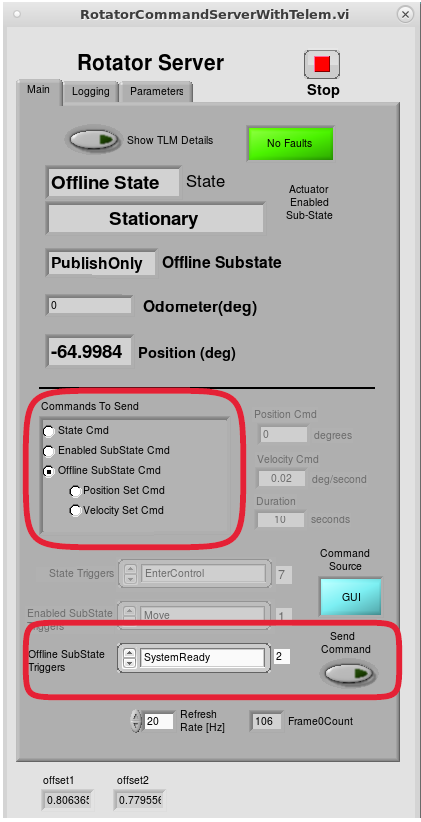
\includegraphics{jira_imgs/1005.png}

      \vspace{\dp0}
      } \end{minipage} \\
      \\ \cdashline{2-3}



      & Expected Result &

      \begin{minipage}[t]{13cm}{\footnotesize
      The system transitions from the OfflineState/PublishOnly substate to the
OfflineState/AvailableState substate.\\
~\\
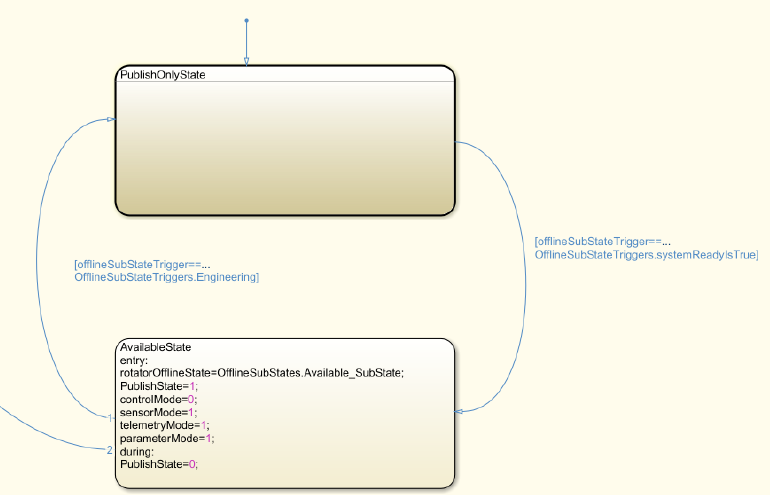
\includegraphics[width=4.6875in,height=\textheight]{jira_imgs/1007.png}

      \vspace{\dp0}
      } \end{minipage} \\
      \\ \cdashline{2-3}

      & \begin{minipage}[t]{2cm}{Actual\\ Result}\end{minipage}   & 
      \begin{minipage}[t]{13cm}{\footnotesize
      
      \vspace{\dp0}
      } \end{minipage} \\
      \\ \cdashline{2-3}


      & Status          & Not Executed \\ \hline

      4 & Description &

      \begin{minipage}[t]{13cm}{\footnotesize
      \textbf{OFFLINESTATE -\textgreater{} STANDBYSTATE}\\
Click on the State Command field in the Commands to Send section.\\
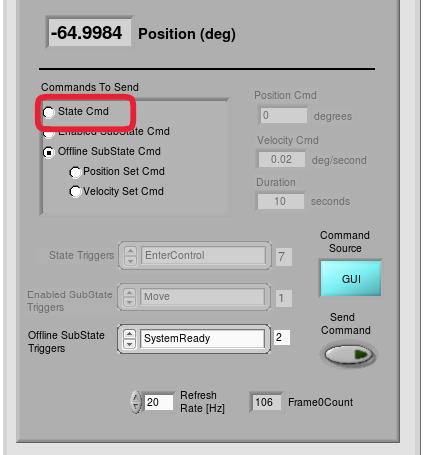
\includegraphics{jira_imgs/1030.png}

      \vspace{\dp0}
      } \end{minipage} \\
      \\ \cdashline{2-3}



      & Expected Result &

      \begin{minipage}[t]{13cm}{\footnotesize
      The system transitions into the StandbyState and the primary state
display box at the top of the Main tab says Standby State.\\
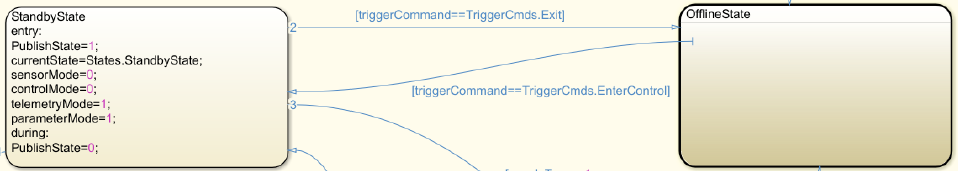
\includegraphics[width=4.6875in,height=\textheight]{jira_imgs/1018.png}

      \vspace{\dp0}
      } \end{minipage} \\
      \\ \cdashline{2-3}

      & \begin{minipage}[t]{2cm}{Actual\\ Result}\end{minipage}   & 
      \begin{minipage}[t]{13cm}{\footnotesize
      
      \vspace{\dp0}
      } \end{minipage} \\
      \\ \cdashline{2-3}


      & Status          & Not Executed \\ \hline

      5 & Description &

      \begin{minipage}[t]{13cm}{\footnotesize
      \textbf{STANDBYSTATE -\textgreater{} DISABLEDSTATE}\\
From the StandbyState, send a start command.

      \vspace{\dp0}
      } \end{minipage} \\
      \\ \cdashline{2-3}



      & Expected Result &

      \begin{minipage}[t]{13cm}{\footnotesize
      The system transitions into DisabledState and the current configuration
parameters are maintained from the default parameters or from the
previous DDS start command.~\\
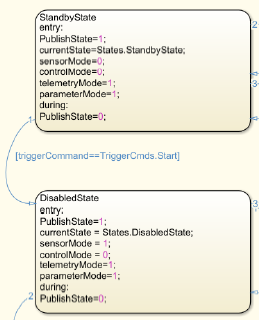
\includegraphics{jira_imgs/1019.png}\\
If the configuration file is invalid or out of range, the system will
transition into a Fault State

      \vspace{\dp0}
      } \end{minipage} \\
      \\ \cdashline{2-3}

      & \begin{minipage}[t]{2cm}{Actual\\ Result}\end{minipage}   & 
      \begin{minipage}[t]{13cm}{\footnotesize
      
      \vspace{\dp0}
      } \end{minipage} \\
      \\ \cdashline{2-3}


      & Status          & Not Executed \\ \hline

      6 & Description &

      \begin{minipage}[t]{13cm}{\footnotesize
      \textbf{DISABLEDSTATE -\textgreater{} ENABLEDSTATE}\\
From the DisabledState, send an Enable state.

      \vspace{\dp0}
      } \end{minipage} \\
      \\ \cdashline{2-3}



      & Expected Result &

      \begin{minipage}[t]{13cm}{\footnotesize
      The system transitions into the EnabledState/Stationary substate, the
motor drives are enabled, and motion can be commanded.\\
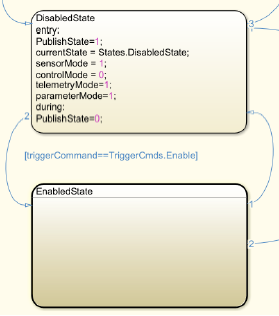
\includegraphics{jira_imgs/1020.png}\\

      \vspace{\dp0}
      } \end{minipage} \\
      \\ \cdashline{2-3}

      & \begin{minipage}[t]{2cm}{Actual\\ Result}\end{minipage}   & 
      \begin{minipage}[t]{13cm}{\footnotesize
      
      \vspace{\dp0}
      } \end{minipage} \\
      \\ \cdashline{2-3}


      & Status          & Not Executed \\ \hline

      7 & Description &

      \begin{minipage}[t]{13cm}{\footnotesize
      \textbf{FAULTSTATE}\\
If a Fault occurs in any of the other states, the system will
automatically transition to the Fault State. While in the Fault state,
send a clearError command.\\
{Note:} If the fault that occurs goes through the interlock system,
reset the safety relay switch and send a clearError command.

      \vspace{\dp0}
      } \end{minipage} \\
      \\ \cdashline{2-3}



      & Expected Result &

      \begin{minipage}[t]{13cm}{\footnotesize
      The system transitions back to the OfflineState/PublishOnly substate.
(Go back to Step 3)\\
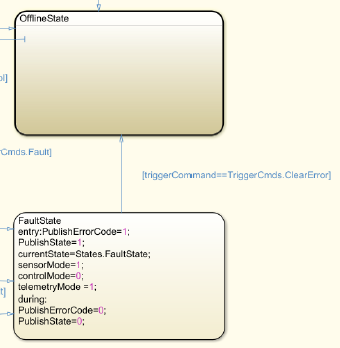
\includegraphics{jira_imgs/1021.png}

      \vspace{\dp0}
      } \end{minipage} \\
      \\ \cdashline{2-3}

      & \begin{minipage}[t]{2cm}{Actual\\ Result}\end{minipage}   & 
      \begin{minipage}[t]{13cm}{\footnotesize
      
      \vspace{\dp0}
      } \end{minipage} \\
      \\ \cdashline{2-3}


      & Status          & Not Executed \\ \hline

      8 & Description &

      \begin{minipage}[t]{13cm}{\footnotesize
      \textbf{Section 3.2.1 of the attached Software Acceptance Test
Procedure\\
Test Sequence \#1 - PositionSet and Move Commands}\\
~\\
In the Enabled/Stationary state, send a positionSet command of 12 deg.

      \vspace{\dp0}
      } \end{minipage} \\
      \\ \cdashline{2-3}



      & Expected Result &

      \begin{minipage}[t]{13cm}{\footnotesize
      Confirm that the rotator does not move.

      \vspace{\dp0}
      } \end{minipage} \\
      \\ \cdashline{2-3}

      & \begin{minipage}[t]{2cm}{Actual\\ Result}\end{minipage}   & 
      \begin{minipage}[t]{13cm}{\footnotesize
      
      \vspace{\dp0}
      } \end{minipage} \\
      \\ \cdashline{2-3}


      & Status          & Not Executed \\ \hline

      9 & Description &

      \begin{minipage}[t]{13cm}{\footnotesize
      Send a positionSet command of 15deg.

      \vspace{\dp0}
      } \end{minipage} \\
      \\ \cdashline{2-3}



      & Expected Result &

      \begin{minipage}[t]{13cm}{\footnotesize
      Confirm that the rotator does not move.

      \vspace{\dp0}
      } \end{minipage} \\
      \\ \cdashline{2-3}

      & \begin{minipage}[t]{2cm}{Actual\\ Result}\end{minipage}   & 
      \begin{minipage}[t]{13cm}{\footnotesize
      
      \vspace{\dp0}
      } \end{minipage} \\
      \\ \cdashline{2-3}


      & Status          & Not Executed \\ \hline

      10 & Description &

      \begin{minipage}[t]{13cm}{\footnotesize
      Send a move command.

      \vspace{\dp0}
      } \end{minipage} \\
      \\ \cdashline{2-3}



      & Expected Result &

      \begin{minipage}[t]{13cm}{\footnotesize
      Confirm that the rotator moves to 15 deg.

      \vspace{\dp0}
      } \end{minipage} \\
      \\ \cdashline{2-3}

      & \begin{minipage}[t]{2cm}{Actual\\ Result}\end{minipage}   & 
      \begin{minipage}[t]{13cm}{\footnotesize
      
      \vspace{\dp0}
      } \end{minipage} \\
      \\ \cdashline{2-3}


      & Status          & Not Executed \\ \hline

      11 & Description &

      \begin{minipage}[t]{13cm}{\footnotesize
      \textbf{Section 3.2.1 of the attached Software Acceptance Test
Procedure\\
Test Sequence \#2 - StopCommand}\\
~\\
In the Enabled/Stationary state, send a positionSet command of 50 deg.

      \vspace{\dp0}
      } \end{minipage} \\
      \\ \cdashline{2-3}



      & Expected Result &

      \begin{minipage}[t]{13cm}{\footnotesize
      Confirm that the rotator does not move.

      \vspace{\dp0}
      } \end{minipage} \\
      \\ \cdashline{2-3}

      & \begin{minipage}[t]{2cm}{Actual\\ Result}\end{minipage}   & 
      \begin{minipage}[t]{13cm}{\footnotesize
      
      \vspace{\dp0}
      } \end{minipage} \\
      \\ \cdashline{2-3}


      & Status          & Not Executed \\ \hline

      12 & Description &

      \begin{minipage}[t]{13cm}{\footnotesize
      Send a move command.

      \vspace{\dp0}
      } \end{minipage} \\
      \\ \cdashline{2-3}



      & Expected Result &

      \begin{minipage}[t]{13cm}{\footnotesize
      The rotator starts it's rotation.

      \vspace{\dp0}
      } \end{minipage} \\
      \\ \cdashline{2-3}

      & \begin{minipage}[t]{2cm}{Actual\\ Result}\end{minipage}   & 
      \begin{minipage}[t]{13cm}{\footnotesize
      
      \vspace{\dp0}
      } \end{minipage} \\
      \\ \cdashline{2-3}


      & Status          & Not Executed \\ \hline

      13 & Description &

      \begin{minipage}[t]{13cm}{\footnotesize
      While the rotator is still moving, send a Stop command.

      \vspace{\dp0}
      } \end{minipage} \\
      \\ \cdashline{2-3}



      & Expected Result &

      \begin{minipage}[t]{13cm}{\footnotesize
      Confirm that the system quickly comes to a stop before reaching the 50
deg position.

      \vspace{\dp0}
      } \end{minipage} \\
      \\ \cdashline{2-3}

      & \begin{minipage}[t]{2cm}{Actual\\ Result}\end{minipage}   & 
      \begin{minipage}[t]{13cm}{\footnotesize
      
      \vspace{\dp0}
      } \end{minipage} \\
      \\ \cdashline{2-3}


      & Status          & Not Executed \\ \hline

      14 & Description &

      \begin{minipage}[t]{13cm}{\footnotesize
      Send a positionSet command of 60 deg followed by a move command.

      \vspace{\dp0}
      } \end{minipage} \\
      \\ \cdashline{2-3}



      & Expected Result &

      \begin{minipage}[t]{13cm}{\footnotesize
      Confirm the rotator moves to the commanded position following the
previous stop command.

      \vspace{\dp0}
      } \end{minipage} \\
      \\ \cdashline{2-3}

      & \begin{minipage}[t]{2cm}{Actual\\ Result}\end{minipage}   & 
      \begin{minipage}[t]{13cm}{\footnotesize
      
      \vspace{\dp0}
      } \end{minipage} \\
      \\ \cdashline{2-3}


      & Status          & Not Executed \\ \hline

      15 & Description &

      \begin{minipage}[t]{13cm}{\footnotesize
      \textbf{Section 3.2.1 of the attached Software Acceptance Test
Procedure\\
Test Sequence \#3 - VelocitySet and MoveConstantVelocity Commands}\\
~\\
In the Enabled/Stationary state, send a velocitySet command of 0.01
deg/s and 15 seconds.

      \vspace{\dp0}
      } \end{minipage} \\
      \\ \cdashline{2-3}



      & Expected Result &

      \begin{minipage}[t]{13cm}{\footnotesize
      Confirm that the rotator does not move.

      \vspace{\dp0}
      } \end{minipage} \\
      \\ \cdashline{2-3}

      & \begin{minipage}[t]{2cm}{Actual\\ Result}\end{minipage}   & 
      \begin{minipage}[t]{13cm}{\footnotesize
      
      \vspace{\dp0}
      } \end{minipage} \\
      \\ \cdashline{2-3}


      & Status          & Not Executed \\ \hline

      16 & Description &

      \begin{minipage}[t]{13cm}{\footnotesize
      Send a velocitySet command of 0.02 deg/s and 10 seconds.

      \vspace{\dp0}
      } \end{minipage} \\
      \\ \cdashline{2-3}



      & Expected Result &

      \begin{minipage}[t]{13cm}{\footnotesize
      Confirm that the rotator does not move.

      \vspace{\dp0}
      } \end{minipage} \\
      \\ \cdashline{2-3}

      & \begin{minipage}[t]{2cm}{Actual\\ Result}\end{minipage}   & 
      \begin{minipage}[t]{13cm}{\footnotesize
      
      \vspace{\dp0}
      } \end{minipage} \\
      \\ \cdashline{2-3}


      & Status          & Not Executed \\ \hline

      17 & Description &

      \begin{minipage}[t]{13cm}{\footnotesize
      Send a moveConstantVelocity command.

      \vspace{\dp0}
      } \end{minipage} \\
      \\ \cdashline{2-3}



      & Expected Result &

      \begin{minipage}[t]{13cm}{\footnotesize
      Confirm that the rotator moves approximately 0.2 degrees total over 10
seconds before coming to a stop and transitioning back to
enabled/stationary state.

      \vspace{\dp0}
      } \end{minipage} \\
      \\ \cdashline{2-3}

      & \begin{minipage}[t]{2cm}{Actual\\ Result}\end{minipage}   & 
      \begin{minipage}[t]{13cm}{\footnotesize
      
      \vspace{\dp0}
      } \end{minipage} \\
      \\ \cdashline{2-3}


      & Status          & Not Executed \\ \hline

      18 & Description &

      \begin{minipage}[t]{13cm}{\footnotesize
      \textbf{Test of the Velocity Limit}\\
~\\
In the enabled/stationary state, send a velocitySet command of 4deg/s
and 5 seconds through the EUI.

      \vspace{\dp0}
      } \end{minipage} \\
      \\ \cdashline{2-3}



      & Expected Result &

      \begin{minipage}[t]{13cm}{\footnotesize
      The EUI does not allow for any value higher than 3.5 deg/s as an input
for the velocitySet command.\\
\emph{Note: If the EUI does not reject the velocitySet command, go to
Step 12.}

      \vspace{\dp0}
      } \end{minipage} \\
      \\ \cdashline{2-3}

      & \begin{minipage}[t]{2cm}{Actual\\ Result}\end{minipage}   & 
      \begin{minipage}[t]{13cm}{\footnotesize
      
      \vspace{\dp0}
      } \end{minipage} \\
      \\ \cdashline{2-3}


      & Status          & Not Executed \\ \hline

      19 & Description &

      \begin{minipage}[t]{13cm}{\footnotesize
      \textbf{\emph{\textless{}Conditional Step\textgreater{}}}\\
~\\
If the EUI accepts the value of 4deg/s and 5 seconds, send a move
command.

      \vspace{\dp0}
      } \end{minipage} \\
      \\ \cdashline{2-3}



      & Expected Result &

      \begin{minipage}[t]{13cm}{\footnotesize
      If the rotator does not ignore the velocitySet command, the rotator does
not move at a higher velocity than the velocity limit of 3.5 deg/s.

      \vspace{\dp0}
      } \end{minipage} \\
      \\ \cdashline{2-3}

      & \begin{minipage}[t]{2cm}{Actual\\ Result}\end{minipage}   & 
      \begin{minipage}[t]{13cm}{\footnotesize
      
      \vspace{\dp0}
      } \end{minipage} \\
      \\ \cdashline{2-3}


      & Status          & Not Executed \\ \hline

      20 & Description &

      \begin{minipage}[t]{13cm}{\footnotesize
      Perform a shutdown of the rotator.

      \vspace{\dp0}
      } \end{minipage} \\
      \\ \cdashline{2-3}



      & Expected Result &

      \begin{minipage}[t]{13cm}{\footnotesize
      Rotator is shutdown.

      \vspace{\dp0}
      } \end{minipage} \\
      \\ \cdashline{2-3}

      & \begin{minipage}[t]{2cm}{Actual\\ Result}\end{minipage}   & 
      \begin{minipage}[t]{13cm}{\footnotesize
      
      \vspace{\dp0}
      } \end{minipage} \\
      \\ \cdashline{2-3}


      & Status          & Not Executed \\ \hline

      21 & Description &

      \begin{minipage}[t]{13cm}{\footnotesize
      \textbf{Section 3.3.1 of the attached Software Acceptance Test
Procedure}\\
\textbf{Actions on State Commands\\
}~\\
Startup the rotator.

      \vspace{\dp0}
      } \end{minipage} \\
      \\ \cdashline{2-3}



      & Expected Result &

      \begin{minipage}[t]{13cm}{\footnotesize
      Confirm that the rotator starts in the Offline/PublishOnly state.

      \vspace{\dp0}
      } \end{minipage} \\
      \\ \cdashline{2-3}

      & \begin{minipage}[t]{2cm}{Actual\\ Result}\end{minipage}   & 
      \begin{minipage}[t]{13cm}{\footnotesize
      
      \vspace{\dp0}
      } \end{minipage} \\
      \\ \cdashline{2-3}


      & Status          & Not Executed \\ \hline

      22 & Description &

      \begin{minipage}[t]{13cm}{\footnotesize
      Send an Offline substate trigger of systemReady.

      \vspace{\dp0}
      } \end{minipage} \\
      \\ \cdashline{2-3}



      & Expected Result &

      \begin{minipage}[t]{13cm}{\footnotesize
      Confirm system goes into Offline/Available substate.

      \vspace{\dp0}
      } \end{minipage} \\
      \\ \cdashline{2-3}

      & \begin{minipage}[t]{2cm}{Actual\\ Result}\end{minipage}   & 
      \begin{minipage}[t]{13cm}{\footnotesize
      
      \vspace{\dp0}
      } \end{minipage} \\
      \\ \cdashline{2-3}


      & Status          & Not Executed \\ \hline

      23 & Description &

      \begin{minipage}[t]{13cm}{\footnotesize
      Send an EnterControl trigger.

      \vspace{\dp0}
      } \end{minipage} \\
      \\ \cdashline{2-3}



      & Expected Result &

      \begin{minipage}[t]{13cm}{\footnotesize
      Confirm the system transitions from Offline/Available to Standby state.

      \vspace{\dp0}
      } \end{minipage} \\
      \\ \cdashline{2-3}

      & \begin{minipage}[t]{2cm}{Actual\\ Result}\end{minipage}   & 
      \begin{minipage}[t]{13cm}{\footnotesize
      
      \vspace{\dp0}
      } \end{minipage} \\
      \\ \cdashline{2-3}


      & Status          & Not Executed \\ \hline

      24 & Description &

      \begin{minipage}[t]{13cm}{\footnotesize
      Send a Start trigger.

      \vspace{\dp0}
      } \end{minipage} \\
      \\ \cdashline{2-3}



      & Expected Result &

      \begin{minipage}[t]{13cm}{\footnotesize
      Confirm the system transitions from Standby to Disabled state.

      \vspace{\dp0}
      } \end{minipage} \\
      \\ \cdashline{2-3}

      & \begin{minipage}[t]{2cm}{Actual\\ Result}\end{minipage}   & 
      \begin{minipage}[t]{13cm}{\footnotesize
      
      \vspace{\dp0}
      } \end{minipage} \\
      \\ \cdashline{2-3}


      & Status          & Not Executed \\ \hline

      25 & Description &

      \begin{minipage}[t]{13cm}{\footnotesize
      Send an Enable trigger.

      \vspace{\dp0}
      } \end{minipage} \\
      \\ \cdashline{2-3}



      & Expected Result &

      \begin{minipage}[t]{13cm}{\footnotesize
      Confirm the system transitions from Disabled to Enabled state.

      \vspace{\dp0}
      } \end{minipage} \\
      \\ \cdashline{2-3}

      & \begin{minipage}[t]{2cm}{Actual\\ Result}\end{minipage}   & 
      \begin{minipage}[t]{13cm}{\footnotesize
      
      \vspace{\dp0}
      } \end{minipage} \\
      \\ \cdashline{2-3}


      & Status          & Not Executed \\ \hline

      26 & Description &

      \begin{minipage}[t]{13cm}{\footnotesize
      Send a Disable trigger.

      \vspace{\dp0}
      } \end{minipage} \\
      \\ \cdashline{2-3}



      & Expected Result &

      \begin{minipage}[t]{13cm}{\footnotesize
      Confirm the system transitions from Enabled to Disabled state.

      \vspace{\dp0}
      } \end{minipage} \\
      \\ \cdashline{2-3}

      & \begin{minipage}[t]{2cm}{Actual\\ Result}\end{minipage}   & 
      \begin{minipage}[t]{13cm}{\footnotesize
      
      \vspace{\dp0}
      } \end{minipage} \\
      \\ \cdashline{2-3}


      & Status          & Not Executed \\ \hline

      27 & Description &

      \begin{minipage}[t]{13cm}{\footnotesize
      Send a Standby trigger.\\
~\\

      \vspace{\dp0}
      } \end{minipage} \\
      \\ \cdashline{2-3}



      & Expected Result &

      \begin{minipage}[t]{13cm}{\footnotesize
      Confirm the system transitions from Disabled state to Standby state.

      \vspace{\dp0}
      } \end{minipage} \\
      \\ \cdashline{2-3}

      & \begin{minipage}[t]{2cm}{Actual\\ Result}\end{minipage}   & 
      \begin{minipage}[t]{13cm}{\footnotesize
      
      \vspace{\dp0}
      } \end{minipage} \\
      \\ \cdashline{2-3}


      & Status          & Not Executed \\ \hline

      28 & Description &

      \begin{minipage}[t]{13cm}{\footnotesize
      Send a exitControl trigger.

      \vspace{\dp0}
      } \end{minipage} \\
      \\ \cdashline{2-3}



      & Expected Result &

      \begin{minipage}[t]{13cm}{\footnotesize
      Confirm the system transitions from Standby state to Offline state.

      \vspace{\dp0}
      } \end{minipage} \\
      \\ \cdashline{2-3}

      & \begin{minipage}[t]{2cm}{Actual\\ Result}\end{minipage}   & 
      \begin{minipage}[t]{13cm}{\footnotesize
      
      \vspace{\dp0}
      } \end{minipage} \\
      \\ \cdashline{2-3}


      & Status          & Not Executed \\ \hline

      29 & Description &

      \begin{minipage}[t]{13cm}{\footnotesize
      Return to the Enabled state and trip the safety interlock switch.

      \vspace{\dp0}
      } \end{minipage} \\
      \\ \cdashline{2-3}



      & Expected Result &

      \begin{minipage}[t]{13cm}{\footnotesize
      Confirm the system transitions to Fault state.

      \vspace{\dp0}
      } \end{minipage} \\
      \\ \cdashline{2-3}

      & \begin{minipage}[t]{2cm}{Actual\\ Result}\end{minipage}   & 
      \begin{minipage}[t]{13cm}{\footnotesize
      
      \vspace{\dp0}
      } \end{minipage} \\
      \\ \cdashline{2-3}


      & Status          & Not Executed \\ \hline

      30 & Description &

      \begin{minipage}[t]{13cm}{\footnotesize
      Reset the safety interlock and send a ClearError trigger.

      \vspace{\dp0}
      } \end{minipage} \\
      \\ \cdashline{2-3}



      & Expected Result &

      \begin{minipage}[t]{13cm}{\footnotesize
      Confirm the system transitions from Fault state to Offline state.

      \vspace{\dp0}
      } \end{minipage} \\
      \\ \cdashline{2-3}

      & \begin{minipage}[t]{2cm}{Actual\\ Result}\end{minipage}   & 
      \begin{minipage}[t]{13cm}{\footnotesize
      
      \vspace{\dp0}
      } \end{minipage} \\
      \\ \cdashline{2-3}


      & Status          & Not Executed \\ \hline

      31 & Description &

      \begin{minipage}[t]{13cm}{\footnotesize
      \textbf{Section 5.1 of the attached Software Acceptance Test
Procedure}\\
\textbf{Rotator Events\\
}~\\
In the Enabled state, unplug an encoder cable for one of the rotator
motors.

      \vspace{\dp0}
      } \end{minipage} \\
      \\ \cdashline{2-3}


        & Test Data        &
        \begin{minipage}[t]{13cm}{\smallskip \footnotesize
        \textbf{Deviation:~}Perform the following set of steps using the EUI
instead of the DDS and verify the events are displayed on the EUI.

        \medskip
        } \end{minipage} \\
        \\ \cdashline{2-3}

      & Expected Result &

      \begin{minipage}[t]{13cm}{\footnotesize
      Confirm that a Drive Fault event is created and the system transitions
to Fault state.

      \vspace{\dp0}
      } \end{minipage} \\
      \\ \cdashline{2-3}

      & \begin{minipage}[t]{2cm}{Actual\\ Result}\end{minipage}   & 
      \begin{minipage}[t]{13cm}{\footnotesize
      
      \vspace{\dp0}
      } \end{minipage} \\
      \\ \cdashline{2-3}


      & Status          & Not Executed \\ \hline

      32 & Description &

      \begin{minipage}[t]{13cm}{\footnotesize
      In the Enabled state, unplug a linear encoder cable for the rotator.

      \vspace{\dp0}
      } \end{minipage} \\
      \\ \cdashline{2-3}



      & Expected Result &

      \begin{minipage}[t]{13cm}{\footnotesize
      Confirm that a Linear Encoder Error event is created and the system
transitions to Fault state.

      \vspace{\dp0}
      } \end{minipage} \\
      \\ \cdashline{2-3}

      & \begin{minipage}[t]{2cm}{Actual\\ Result}\end{minipage}   & 
      \begin{minipage}[t]{13cm}{\footnotesize
      
      \vspace{\dp0}
      } \end{minipage} \\
      \\ \cdashline{2-3}


      & Status          & Not Executed \\ \hline

      33 & Description &

      \begin{minipage}[t]{13cm}{\footnotesize
      Set the Following Error Threshold parameter to a very small value
(0.0001 deg or smaller) and send a PositionSet and then Move command.

      \vspace{\dp0}
      } \end{minipage} \\
      \\ \cdashline{2-3}



      & Expected Result &

      \begin{minipage}[t]{13cm}{\footnotesize
      Confirm that a Following Error event is created and the system
transitions to Fault state.

      \vspace{\dp0}
      } \end{minipage} \\
      \\ \cdashline{2-3}

      & \begin{minipage}[t]{2cm}{Actual\\ Result}\end{minipage}   & 
      \begin{minipage}[t]{13cm}{\footnotesize
      
      \vspace{\dp0}
      } \end{minipage} \\
      \\ \cdashline{2-3}


      & Status          & Not Executed \\ \hline

      34 & Description &

      \begin{minipage}[t]{13cm}{\footnotesize
      Activate the positive software limit using a special control program.

      \vspace{\dp0}
      } \end{minipage} \\
      \\ \cdashline{2-3}



      & Expected Result &

      \begin{minipage}[t]{13cm}{\footnotesize
      Confirm that a Positive Limit Switch error message is created and the
system transitions to Fault state.

      \vspace{\dp0}
      } \end{minipage} \\
      \\ \cdashline{2-3}

      & \begin{minipage}[t]{2cm}{Actual\\ Result}\end{minipage}   & 
      \begin{minipage}[t]{13cm}{\footnotesize
      
      \vspace{\dp0}
      } \end{minipage} \\
      \\ \cdashline{2-3}


      & Status          & Not Executed \\ \hline

      35 & Description &

      \begin{minipage}[t]{13cm}{\footnotesize
      Activate the negative software limit using a special control program.

      \vspace{\dp0}
      } \end{minipage} \\
      \\ \cdashline{2-3}



      & Expected Result &

      \begin{minipage}[t]{13cm}{\footnotesize
      Confirm that a Negative Limit Switch error message is created and the
system transitions to Fault State.

      \vspace{\dp0}
      } \end{minipage} \\
      \\ \cdashline{2-3}

      & \begin{minipage}[t]{2cm}{Actual\\ Result}\end{minipage}   & 
      \begin{minipage}[t]{13cm}{\footnotesize
      
      \vspace{\dp0}
      } \end{minipage} \\
      \\ \cdashline{2-3}


      & Status          & Not Executed \\ \hline

      36 & Description &

      \begin{minipage}[t]{13cm}{\footnotesize
      Unplug the Ethercat cable between the control PC and the Copley XE2
drive.\\
~\\

      \vspace{\dp0}
      } \end{minipage} \\
      \\ \cdashline{2-3}



      & Expected Result &

      \begin{minipage}[t]{13cm}{\footnotesize
      Confirm that an Ethercat Problem event is created and the system
transitions to Fault state.

      \vspace{\dp0}
      } \end{minipage} \\
      \\ \cdashline{2-3}

      & \begin{minipage}[t]{2cm}{Actual\\ Result}\end{minipage}   & 
      \begin{minipage}[t]{13cm}{\footnotesize
      
      \vspace{\dp0}
      } \end{minipage} \\
      \\ \cdashline{2-3}


      & Status          & Not Executed \\ \hline

      37 & Description &

      \begin{minipage}[t]{13cm}{\footnotesize
      Perform a shutdown of the rotator.

      \vspace{\dp0}
      } \end{minipage} \\
      \\ \cdashline{2-3}



      & Expected Result &

      \begin{minipage}[t]{13cm}{\footnotesize
      Rotator is shutdown.

      \vspace{\dp0}
      } \end{minipage} \\
      \\ \cdashline{2-3}

      & \begin{minipage}[t]{2cm}{Actual\\ Result}\end{minipage}   & 
      \begin{minipage}[t]{13cm}{\footnotesize
      
      \vspace{\dp0}
      } \end{minipage} \\
      \\ \cdashline{2-3}


      & Status          & Not Executed \\ \hline

      38 & Description &

      \begin{minipage}[t]{13cm}{\footnotesize
      \textbf{Section 5.0 of the attached Software Acceptance Test
Procedure}\\
\textbf{Rotator Telemetry Verification}\\
~\\
Using the EFD, verify that the following telemetry streams were
published at a rate of 20Hz.

\begin{itemize}
\tightlist
\item
  \textbf{rotator\_Application, Demand:} Commanded rotator position in
  degrees.
\item
  \textbf{rotator\_Application, Position:} Actual rotator position in
  degrees.
\item
  \textbf{rotator\_Application, Error:} Indication of a rotator
  following error.
\item
  \textbf{rotator\_Motors, Calibrated:} Encoder readings from each
  rotator motor scaled to degrees of the rotator.
\item
  \textbf{rotator\_Motors, Raw:} Encoder readings from each rotator
  motor in counts.
\item
  \textbf{rotator\_Electrical, CopleyStatusWordDrive:}
\end{itemize}

      \vspace{\dp0}
      } \end{minipage} \\
      \\ \cdashline{2-3}



      & Expected Result &

      \begin{minipage}[t]{13cm}{\footnotesize
      The defined telemetry streams were published to the EFD at 20Hz.

      \vspace{\dp0}
      } \end{minipage} \\
      \\ \cdashline{2-3}

      & \begin{minipage}[t]{2cm}{Actual\\ Result}\end{minipage}   & 
      \begin{minipage}[t]{13cm}{\footnotesize
      
      \vspace{\dp0}
      } \end{minipage} \\
      \\ \cdashline{2-3}


      & Status          & Not Executed \\ \hline

    \end{longtable}


    \paragraph{Test Case LVV-T1576 - Camera Rotator Hardware Functional Re-verification
 }\mbox{}\\

Open  \href{https://jira.lsstcorp.org/secure/Tests.jspa#/testCase/LVV-T1576}{\textit{ LVV-T1576 } }
test case in Jira.

    The objective of this test case is to re-verify the functional
requirements of the camera rotator's hardware, after shipment from the
vendors facility to the Summit, as defined in \citeds{LTS-206}. This test case
will only exercise the functionality that was executed previously and
meets the following criteria:

\begin{itemize}
\tightlist
\item
  Only requires the camera rotator to be operable
\item
  Only requires the vendors EUI software and hardware via local control
\item
  Only requires a laser tracker
\item
  Does \textbf{NOT} require the camera rotator to be loaded with the
  camera simulated mass or actual camera hardware
\end{itemize}

The hardware functional requirements were previously verified during the
test campaign by the vendor at the vendors facility and accepted by LSST
during the Factory Acceptance Test review. The test procedure used
during the vendor's acceptance testing is the \emph{LSST
Hexapods-Rotator Acceptance Test Procedure} which is attached to this
test case. The test steps of this test case reference that document for
the details on how to perform the test in a similar way as was performed
previously and includes deviations to that document due to the
differences in the verification configuration and deviations to
requirements granted to the vendor by LSST.\\
~\\
The \emph{LSST Hexapods-Rotator Acceptance Test Report} has also been
attached to this test case for additional information on how the tests
were performed. The section numbering in this document matches that of
the procedure.\\
~\\
See the attached \emph{LSST Rotator Operator's Manual} for more
information on how to operate the rotator.


    \textbf{ Preconditions}:\\
    {Prior to the execution of this test case to re-verify the Camera
Rotator hardware functional requirements, the following Summit tasks
must be completed:}

\begin{itemize}
\tightlist
\item
  The cables and cabinets have been checked~

  \begin{itemize}
  \tightlist
  \item
    \url{https://jira.lsstcorp.org/browse/SUMMIT-3231}
  \end{itemize}
\item
  Boxes for the hexapod/rotator have been transported to the 3rd level

  \begin{itemize}
  \tightlist
  \item
    \url{https://jira.lsstcorp.org/browse/SUMMIT-3230}
  \end{itemize}
\item
  Test fit Camera Hexapod with Offset

  \begin{itemize}
  \tightlist
  \item
    \url{https://jira.lsstcorp.org/browse/SUMMIT-3293}
  \end{itemize}
\item
  The Hexapod and Rotator have been installed on camera cart

  \begin{itemize}
  \tightlist
  \item
    \url{https://jira.lsstcorp.org/browse/SUMMIT-3224}
  \end{itemize}
\item
  The Camera hexapod/rotator has been connected to the electronics
  cabinets and the connections have been tested

  \begin{itemize}
  \tightlist
  \item
    \url{https://jira.lsstcorp.org/browse/SUMMIT-3294}
  \end{itemize}
\item
  The Offset has been installed on the Integrator

  \begin{itemize}
  \tightlist
  \item
    \url{https://jira.lsstcorp.org/browse/SUMMIT-3281}
  \end{itemize}
\item
  The setup for the laser tracker, current probes and data acquisition
  system has been completed

  \begin{itemize}
  \tightlist
  \item
    \url{https://jira.lsstcorp.org/browse/SUMMIT-3431}
  \end{itemize}
\end{itemize}


    Execution status: {\bf Not Executed }

    Final comment:\\


    Detailed step results:

    \begin{longtable}{p{1cm}p{2cm}p{13cm}}
    \hline
    {Step} & \multicolumn{2}{c}{Description, Results and Status}\\ \hline
      1 & Description &

      \begin{minipage}[t]{13cm}{\footnotesize
      \textbf{STARTING THE EUI}\\
~\\
Double click the Hexapod GUI Viewer desktop icon on the computer.

\begin{itemize}
\tightlist
\item
  This can be done on the Dell Management PC or another computer on the
  same network
\end{itemize}

      \vspace{\dp0}
      } \end{minipage} \\
      \\ \cdashline{2-3}



      & Expected Result &

      \begin{minipage}[t]{13cm}{\footnotesize
      A prompt to enter the password is shown.

      \vspace{\dp0}
      } \end{minipage} \\
      \\ \cdashline{2-3}

      & \begin{minipage}[t]{2cm}{Actual\\ Result}\end{minipage}   & 
      \begin{minipage}[t]{13cm}{\footnotesize
      
      \vspace{\dp0}
      } \end{minipage} \\
      \\ \cdashline{2-3}


      & Status          & Not Executed \\ \hline

      2 & Description &

      \begin{minipage}[t]{13cm}{\footnotesize
      Enter the password "lsst-vnc"

\begin{itemize}
\tightlist
\item
  If the EUI isn't automatically up and running when the VNC opens,
  double click on the CAM\_Hex\_eGUI or M2\_Hex\_eGUI icon on the VNC
  viewer
\end{itemize}

      \vspace{\dp0}
      } \end{minipage} \\
      \\ \cdashline{2-3}



      & Expected Result &

      \begin{minipage}[t]{13cm}{\footnotesize
      The EUI is in the Offline State/PublishOnly substate and is able to
publish through SAL but cannot receive commands.

      \vspace{\dp0}
      } \end{minipage} \\
      \\ \cdashline{2-3}

      & \begin{minipage}[t]{2cm}{Actual\\ Result}\end{minipage}   & 
      \begin{minipage}[t]{13cm}{\footnotesize
      
      \vspace{\dp0}
      } \end{minipage} \\
      \\ \cdashline{2-3}


      & Status          & Not Executed \\ \hline

      3 & Description &

      \begin{minipage}[t]{13cm}{\footnotesize
      \textbf{OFFLINESTATE/AVAILABLESTATE}\\
On the Main tab, select the "Offline SubState Cmd" field in the Commands
to Send section, set the Offline SubState Triggers to "System Ready" and
click on the Send Command button.\\
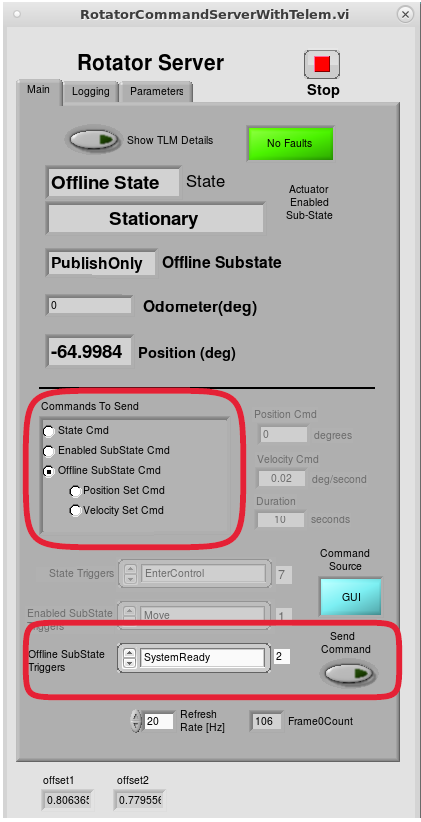
\includegraphics{jira_imgs/1005.png}

      \vspace{\dp0}
      } \end{minipage} \\
      \\ \cdashline{2-3}



      & Expected Result &

      \begin{minipage}[t]{13cm}{\footnotesize
      The system transitions from the OfflineState/PublishOnly substate to the
OfflineState/AvailableState substate.\\
~\\
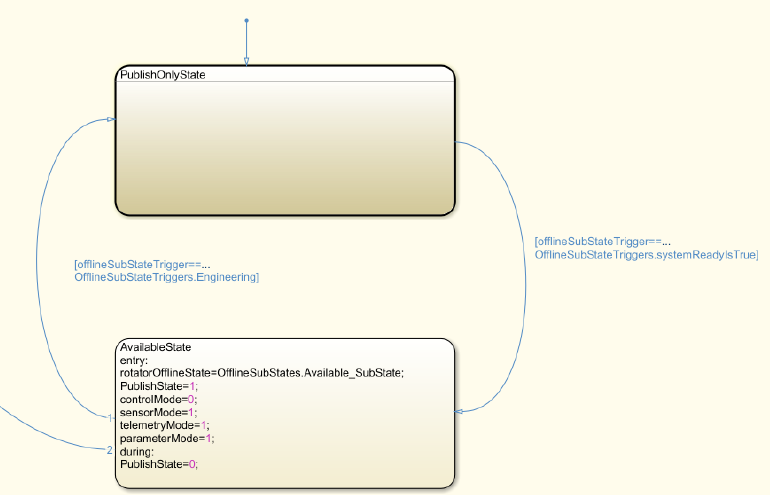
\includegraphics[width=4.6875in,height=\textheight]{jira_imgs/1007.png}

      \vspace{\dp0}
      } \end{minipage} \\
      \\ \cdashline{2-3}

      & \begin{minipage}[t]{2cm}{Actual\\ Result}\end{minipage}   & 
      \begin{minipage}[t]{13cm}{\footnotesize
      
      \vspace{\dp0}
      } \end{minipage} \\
      \\ \cdashline{2-3}


      & Status          & Not Executed \\ \hline

      4 & Description &

      \begin{minipage}[t]{13cm}{\footnotesize
      \textbf{OFFLINESTATE -\textgreater{} STANDBYSTATE}\\
Click on the State Command field in the Commands to Send section.\\
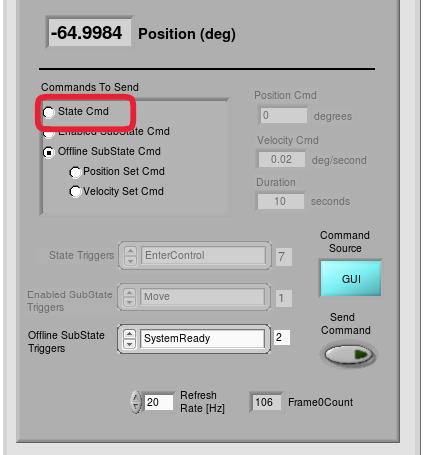
\includegraphics{jira_imgs/1030.png}

      \vspace{\dp0}
      } \end{minipage} \\
      \\ \cdashline{2-3}



      & Expected Result &

      \begin{minipage}[t]{13cm}{\footnotesize
      The system transitions into the StandbyState and the primary state
display box at the top of the Main tab says Standby State.\\
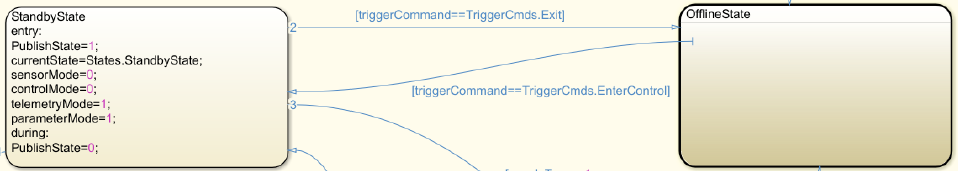
\includegraphics[width=4.6875in,height=\textheight]{jira_imgs/1018.png}

      \vspace{\dp0}
      } \end{minipage} \\
      \\ \cdashline{2-3}

      & \begin{minipage}[t]{2cm}{Actual\\ Result}\end{minipage}   & 
      \begin{minipage}[t]{13cm}{\footnotesize
      
      \vspace{\dp0}
      } \end{minipage} \\
      \\ \cdashline{2-3}


      & Status          & Not Executed \\ \hline

      5 & Description &

      \begin{minipage}[t]{13cm}{\footnotesize
      \textbf{STANDBYSTATE -\textgreater{} DISABLEDSTATE}\\
From the StandbyState, send a start command.

      \vspace{\dp0}
      } \end{minipage} \\
      \\ \cdashline{2-3}



      & Expected Result &

      \begin{minipage}[t]{13cm}{\footnotesize
      The system transitions into DisabledState and the current configuration
parameters are maintained from the default parameters or from the
previous DDS start command.~\\
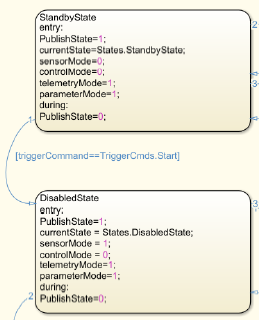
\includegraphics{jira_imgs/1019.png}\\
If the configuration file is invalid or out of range, the system will
transition into a Fault State

      \vspace{\dp0}
      } \end{minipage} \\
      \\ \cdashline{2-3}

      & \begin{minipage}[t]{2cm}{Actual\\ Result}\end{minipage}   & 
      \begin{minipage}[t]{13cm}{\footnotesize
      
      \vspace{\dp0}
      } \end{minipage} \\
      \\ \cdashline{2-3}


      & Status          & Not Executed \\ \hline

      6 & Description &

      \begin{minipage}[t]{13cm}{\footnotesize
      \textbf{DISABLEDSTATE -\textgreater{} ENABLEDSTATE}\\
From the DisabledState, send an Enable state.

      \vspace{\dp0}
      } \end{minipage} \\
      \\ \cdashline{2-3}



      & Expected Result &

      \begin{minipage}[t]{13cm}{\footnotesize
      The system transitions into the EnabledState/Stationary substate, the
motor drives are enabled, and motion can be commanded.\\
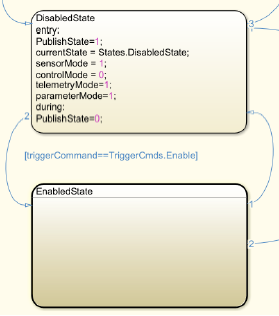
\includegraphics{jira_imgs/1020.png}\\

      \vspace{\dp0}
      } \end{minipage} \\
      \\ \cdashline{2-3}

      & \begin{minipage}[t]{2cm}{Actual\\ Result}\end{minipage}   & 
      \begin{minipage}[t]{13cm}{\footnotesize
      
      \vspace{\dp0}
      } \end{minipage} \\
      \\ \cdashline{2-3}


      & Status          & Not Executed \\ \hline

      7 & Description &

      \begin{minipage}[t]{13cm}{\footnotesize
      \textbf{FAULTSTATE}\\
If a Fault occurs in any of the other states, the system will
automatically transition to the Fault State. While in the Fault state,
send a clearError command.\\
{Note:} If the fault that occurs goes through the interlock system,
reset the safety relay switch and send a clearError command.

      \vspace{\dp0}
      } \end{minipage} \\
      \\ \cdashline{2-3}



      & Expected Result &

      \begin{minipage}[t]{13cm}{\footnotesize
      The system transitions back to the OfflineState/PublishOnly substate.
(Go back to Step 3)\\
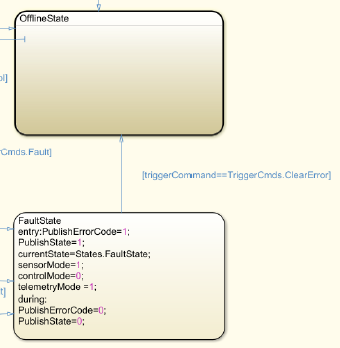
\includegraphics{jira_imgs/1021.png}

      \vspace{\dp0}
      } \end{minipage} \\
      \\ \cdashline{2-3}

      & \begin{minipage}[t]{2cm}{Actual\\ Result}\end{minipage}   & 
      \begin{minipage}[t]{13cm}{\footnotesize
      
      \vspace{\dp0}
      } \end{minipage} \\
      \\ \cdashline{2-3}


      & Status          & Not Executed \\ \hline

      8 & Description &

      \begin{minipage}[t]{13cm}{\footnotesize
      Follow Section 3.4.4 of the LSST Hexapods-Rotator Acceptance Test
Procedure, Sheet 47.

      \vspace{\dp0}
      } \end{minipage} \\
      \\ \cdashline{2-3}


        & Test Data        &
        \begin{minipage}[t]{13cm}{\smallskip \footnotesize
        \textbf{Deviation:} After verifying that the rotator can move through
it's operational range (+/- 90 deg) without triggering any limits,
adjust the software limit to in between the values for the Limit Switch
and End Stop as defined in the table below for SN 02 (taken from
vendor's Acceptance Test Report). Move the rotator to trip the positive
and negative limit switchs.\\
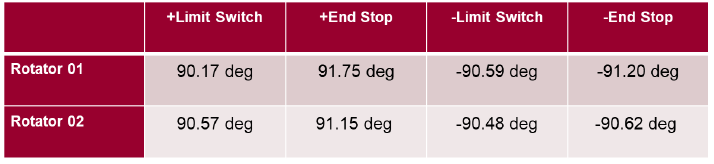
\includegraphics[width=4.6875in,height=\textheight]{jira_imgs/984.png}\\
Do \textbf{NOT} verify the rotator's End Stop hardpoints.

        \medskip
        } \end{minipage} \\
        \\ \cdashline{2-3}

      & Expected Result &

      \begin{minipage}[t]{13cm}{\footnotesize
      \begin{enumerate}
\tightlist
\item
  {The software limit prevents the camera rotator from rotating beyond
  +/-90deg.}
\item
  The limit switch stops the rotator before +/- 92 deg.
\end{enumerate}

      \vspace{\dp0}
      } \end{minipage} \\
      \\ \cdashline{2-3}

      & \begin{minipage}[t]{2cm}{Actual\\ Result}\end{minipage}   & 
      \begin{minipage}[t]{13cm}{\footnotesize
      
      \vspace{\dp0}
      } \end{minipage} \\
      \\ \cdashline{2-3}


      & Status          & Not Executed \\ \hline

      9 & Description &

      \begin{minipage}[t]{13cm}{\footnotesize
      Follow Section 3.4.1 of the LSST Hexapods-Rotator Acceptance Test
Procedure, Sheet 46.

      \vspace{\dp0}
      } \end{minipage} \\
      \\ \cdashline{2-3}



      & Expected Result &

      \begin{minipage}[t]{13cm}{\footnotesize
      The axis of rotation is visually confirmed to be along the z-axis and is
consistent to the results of the initial tests conducted by the vendor
as seen in the LSST Hexapods-Rotator Acceptance Test Report, Sheet 48.

      \vspace{\dp0}
      } \end{minipage} \\
      \\ \cdashline{2-3}

      & \begin{minipage}[t]{2cm}{Actual\\ Result}\end{minipage}   & 
      \begin{minipage}[t]{13cm}{\footnotesize
      
      \vspace{\dp0}
      } \end{minipage} \\
      \\ \cdashline{2-3}


      & Status          & Not Executed \\ \hline

      10 & Description &

      \begin{minipage}[t]{13cm}{\footnotesize
      Follow Section 3.4.2 of the LSST Hexapods-Rotator Acceptance Test
Procedure, Sheet 46 using a laser tracker.

      \vspace{\dp0}
      } \end{minipage} \\
      \\ \cdashline{2-3}


        & Test Data        &
        \begin{minipage}[t]{13cm}{\smallskip \footnotesize
        \textbf{Deviation:} Instead of using 5 different elevation angles, the
test will only be conducted at a 0deg elevation angle

        \medskip
        } \end{minipage} \\
        \\ \cdashline{2-3}

      & Expected Result &

      \begin{minipage}[t]{13cm}{\footnotesize
      The Camera Rotator is tested every 30 degrees across the entire range of
motion and the maximum angle error is found to be less than 0.009
degrees.

      \vspace{\dp0}
      } \end{minipage} \\
      \\ \cdashline{2-3}

      & \begin{minipage}[t]{2cm}{Actual\\ Result}\end{minipage}   & 
      \begin{minipage}[t]{13cm}{\footnotesize
      
      \vspace{\dp0}
      } \end{minipage} \\
      \\ \cdashline{2-3}


      & Status          & Not Executed \\ \hline

      11 & Description &

      \begin{minipage}[t]{13cm}{\footnotesize
      Follow Section 3.4.5.1 of the LSST Hexapods-Rotator Acceptance Test
Procedure, Sheet 48.

      \vspace{\dp0}
      } \end{minipage} \\
      \\ \cdashline{2-3}



      & Expected Result &

      \begin{minipage}[t]{13cm}{\footnotesize
      The Camera Rotator is able to reach the required velocity of 3.5 deg/s
as verified before per the LSST Hexapods-Rotator Acceptance Test Report,
Sheet 50-52

      \vspace{\dp0}
      } \end{minipage} \\
      \\ \cdashline{2-3}

      & \begin{minipage}[t]{2cm}{Actual\\ Result}\end{minipage}   & 
      \begin{minipage}[t]{13cm}{\footnotesize
      
      \vspace{\dp0}
      } \end{minipage} \\
      \\ \cdashline{2-3}


      & Status          & Not Executed \\ \hline

      12 & Description &

      \begin{minipage}[t]{13cm}{\footnotesize
      Follow Section 3.4.5.2 of the LSST Hexapods-Rotator Acceptance Test
Procedure, Sheet 49.

      \vspace{\dp0}
      } \end{minipage} \\
      \\ \cdashline{2-3}



      & Expected Result &

      \begin{minipage}[t]{13cm}{\footnotesize
      The Camera Rotator is able to reach the required acceleration of 1.0
degrees/sec\^{}2 as verified before per the LSST Hexapods\_Rotator
Acceptance Test Report, Sheet 52.

      \vspace{\dp0}
      } \end{minipage} \\
      \\ \cdashline{2-3}

      & \begin{minipage}[t]{2cm}{Actual\\ Result}\end{minipage}   & 
      \begin{minipage}[t]{13cm}{\footnotesize
      
      \vspace{\dp0}
      } \end{minipage} \\
      \\ \cdashline{2-3}


      & Status          & Not Executed \\ \hline

      13 & Description &

      \begin{minipage}[t]{13cm}{\footnotesize
      Follow Section 3.4.5.3 of the LSST Hexapods-Rotator Acceptance Test
Procedure, Sheet 49.

      \vspace{\dp0}
      } \end{minipage} \\
      \\ \cdashline{2-3}


        & Test Data        &
        \begin{minipage}[t]{13cm}{\smallskip \footnotesize
        \textbf{Deviation:~}Steps 7, 8 and 9 (Section 3.4.5.3, 3.4.5.4 and
3.4.5.5) can be tested simultaneously with the same data.

        \medskip
        } \end{minipage} \\
        \\ \cdashline{2-3}

      & Expected Result &

      \begin{minipage}[t]{13cm}{\footnotesize
      The initial result of the test (as seen in LSST Hexapods\_Rotator
Acceptance Test Report, Sheet 52-54) found that the requirement was not
met, but was accepted per deviation request
\url{https://jira.lsstcorp.org/browse/LVV-7218}\emph{. The
re-verification only needs to meet the values approved in the
deviation.\\
}

      \vspace{\dp0}
      } \end{minipage} \\
      \\ \cdashline{2-3}

      & \begin{minipage}[t]{2cm}{Actual\\ Result}\end{minipage}   & 
      \begin{minipage}[t]{13cm}{\footnotesize
      
      \vspace{\dp0}
      } \end{minipage} \\
      \\ \cdashline{2-3}


      & Status          & Not Executed \\ \hline

      14 & Description &

      \begin{minipage}[t]{13cm}{\footnotesize
      Follow Section 3.4.5.4 of the LSST Hexapods-Rotator Acceptance Test
Procedure, Sheet 49.

      \vspace{\dp0}
      } \end{minipage} \\
      \\ \cdashline{2-3}


        & Test Data        &
        \begin{minipage}[t]{13cm}{\smallskip \footnotesize
        \textbf{Deviation:~}Perform this step at a 0 degree elevation angle
instead of the 90 degree angle listed in the procedure and use the same
data used in Step 7.~

        \medskip
        } \end{minipage} \\
        \\ \cdashline{2-3}

      & Expected Result &

      \begin{minipage}[t]{13cm}{\footnotesize
      The maximum radial displacement is measured to be under 50 microns as
previously verified per LSST Hexapods\_Rotator Acceptance Test Report,
Sheet 54.

      \vspace{\dp0}
      } \end{minipage} \\
      \\ \cdashline{2-3}

      & \begin{minipage}[t]{2cm}{Actual\\ Result}\end{minipage}   & 
      \begin{minipage}[t]{13cm}{\footnotesize
      
      \vspace{\dp0}
      } \end{minipage} \\
      \\ \cdashline{2-3}


      & Status          & Not Executed \\ \hline

      15 & Description &

      \begin{minipage}[t]{13cm}{\footnotesize
      Follow Section 3.4.5.5 of the LSST Hexapods-Rotator Acceptance Test
Procedure, Sheet 50.

      \vspace{\dp0}
      } \end{minipage} \\
      \\ \cdashline{2-3}


        & Test Data        &
        \begin{minipage}[t]{13cm}{\smallskip \footnotesize
        \textbf{Deviation:~}Perform this step at a 0 degree elevation angle
instead of the 90 degree angle listed in the procedure and use the same
data used in Step 7.~

        \medskip
        } \end{minipage} \\
        \\ \cdashline{2-3}

      & Expected Result &

      \begin{minipage}[t]{13cm}{\footnotesize
      {The maximum radial displacement is measured to be under 100 microns as
previously verified per LSST Hexapods\_Rotator Acceptance Test Report,
Sheet 55. }

      \vspace{\dp0}
      } \end{minipage} \\
      \\ \cdashline{2-3}

      & \begin{minipage}[t]{2cm}{Actual\\ Result}\end{minipage}   & 
      \begin{minipage}[t]{13cm}{\footnotesize
      
      \vspace{\dp0}
      } \end{minipage} \\
      \\ \cdashline{2-3}


      & Status          & Not Executed \\ \hline

      16 & Description &

      \begin{minipage}[t]{13cm}{\footnotesize
      Follow Section 3.4.5.6 of the LSST Hexapods-Rotator Acceptance Test
Procedure, Sheet 50.

      \vspace{\dp0}
      } \end{minipage} \\
      \\ \cdashline{2-3}


        & Test Data        &
        \begin{minipage}[t]{13cm}{\smallskip \footnotesize
        \textbf{Deviation:} This will be done with a laser tracker knowing that
we will not be able to measure as low as 2 microns.~

        \medskip
        } \end{minipage} \\
        \\ \cdashline{2-3}

      & Expected Result &

      \begin{minipage}[t]{13cm}{\footnotesize
      {Since the error cannot be measured up to 2 microns, the camera
rotator's accuracy is found to be as good as the laser tracker's
accuracy.}

      \vspace{\dp0}
      } \end{minipage} \\
      \\ \cdashline{2-3}

      & \begin{minipage}[t]{2cm}{Actual\\ Result}\end{minipage}   & 
      \begin{minipage}[t]{13cm}{\footnotesize
      
      \vspace{\dp0}
      } \end{minipage} \\
      \\ \cdashline{2-3}


      & Status          & Not Executed \\ \hline

      17 & Description &

      \begin{minipage}[t]{13cm}{\footnotesize
      To verify 3.4.6.1, follow Section 3.4.6.2 of the LSST Hexapods-Rotator
Acceptance Test Procedure, Sheet 50-52.

      \vspace{\dp0}
      } \end{minipage} \\
      \\ \cdashline{2-3}


        & Test Data        &
        \begin{minipage}[t]{13cm}{\smallskip \footnotesize
        \textbf{Deviation:} Steps 10 and 11 (Section 3.4.6.1 and 3.4.6.2) will
be tested simultaneously.\\
We will be testing all speeds from 0.005 to 0.068deg/s just like in LSST
Hexapods-Rotator Acceptance Test Report Sheets 57-64. However, we will
only be using the encoder (no laser interferometer) and one elevation
angle (0 Deg El) to verify.

        \medskip
        } \end{minipage} \\
        \\ \cdashline{2-3}

      & Expected Result &

      \begin{minipage}[t]{13cm}{\footnotesize
      \begin{enumerate}
\tightlist
\item
  The SN02 Rotator is found to be able to reach all of the testing
  speeds from 0.005 to 0.068deg/s with a zero degree elevation angle.~
\item
  The SN02 Rotator's Tracking Accuracy is recorded for all tracking
  velocities from 0.05deg/s to 0.068deg/s with a zero degree elevation
  angle and is found to have a position error equal or better than 0.1
  arcs seconds RMS.
\end{enumerate}

      \vspace{\dp0}
      } \end{minipage} \\
      \\ \cdashline{2-3}

      & \begin{minipage}[t]{2cm}{Actual\\ Result}\end{minipage}   & 
      \begin{minipage}[t]{13cm}{\footnotesize
      
      \vspace{\dp0}
      } \end{minipage} \\
      \\ \cdashline{2-3}


      & Status          & Not Executed \\ \hline

      18 & Description &

      \begin{minipage}[t]{13cm}{\footnotesize
      Follow Section 3.4.6.6 of the LSST Hexapods-Rotator Acceptance Test
Procedure, Sheet 53

      \vspace{\dp0}
      } \end{minipage} \\
      \\ \cdashline{2-3}


        & Test Data        &
        \begin{minipage}[t]{13cm}{\smallskip \footnotesize
        \textbf{Deviation:~}This will only be conducted at 0 deg elevation angle
since it is on the camera cart.

        \medskip
        } \end{minipage} \\
        \\ \cdashline{2-3}

      & Expected Result &

      \begin{minipage}[t]{13cm}{\footnotesize
      By checking the current of the system, the heat dissipation for the
rotator is verified to be less than 40W.

      \vspace{\dp0}
      } \end{minipage} \\
      \\ \cdashline{2-3}

      & \begin{minipage}[t]{2cm}{Actual\\ Result}\end{minipage}   & 
      \begin{minipage}[t]{13cm}{\footnotesize
      
      \vspace{\dp0}
      } \end{minipage} \\
      \\ \cdashline{2-3}


      & Status          & Not Executed \\ \hline

      19 & Description &

      \begin{minipage}[t]{13cm}{\footnotesize
      Follow Section 3.4.9 of the LSST Hexapods-Rotator Acceptance Test
Procedure, Sheet 54.

      \vspace{\dp0}
      } \end{minipage} \\
      \\ \cdashline{2-3}



      & Expected Result &

      \begin{minipage}[t]{13cm}{\footnotesize
      The locking pin is demonstrated to be able to engage at 15 deg intervals
throughout the entire rotator range while the camera hexapod/rotator is
installed on the camera cart.

      \vspace{\dp0}
      } \end{minipage} \\
      \\ \cdashline{2-3}

      & \begin{minipage}[t]{2cm}{Actual\\ Result}\end{minipage}   & 
      \begin{minipage}[t]{13cm}{\footnotesize
      
      \vspace{\dp0}
      } \end{minipage} \\
      \\ \cdashline{2-3}


      & Status          & Not Executed \\ \hline

    \end{longtable}


\newpage
\appendix
%Make sure lsst-texmf/bin/generateAcronyms.py is in your path
\section{Acronyms used in this document}\label{sec:acronyms}
\addtocounter{table}{-1}
\begin{longtable}{p{0.145\textwidth}p{0.8\textwidth}}\hline
\textbf{Acronym} & \textbf{Description}  \\\hline

EFD & Engineering and Facility Database \\\hline
GUI & Graphical User Interface \\\hline
LSST & Large Synoptic Survey Telescope \\\hline
PMCS & Project Management Controls System \\\hline
RMS & Root-Mean-Square \\\hline
SLAC & SLAC National Accelerator Laboratory (formerly Stanford Linear Accelerator Center; SLAC is now no longer an acronym) \\\hline
\end{longtable}


\end{document}
